\documentclass[11pt,a4paper]{article}

% ------- Encoding & fonts -------
\usepackage[utf8]{inputenc}
\usepackage[T1]{fontenc}
\usepackage{lmodern}
\usepackage{microtype}
% ---- Pipeline diagram ----
\usepackage{tikz}
\usetikzlibrary{arrows.meta,positioning,shapes.geometric,shapes.misc}

% ------- Layout & color & links -------
\usepackage[a4paper,margin=1in]{geometry}
\usepackage{hyperref}
\hypersetup{colorlinks=true,linkcolor=black,citecolor=black,urlcolor=blue}

% ------- Tables & formatting -------
\usepackage{booktabs}
\usepackage{longtable}
\usepackage{array}
\usepackage{ragged2e}
\usepackage{enumitem}
\usepackage{graphicx}
\usepackage{amsmath,amssymb}
\usepackage{footnote}
\usepackage{tabularx}
\makesavenoteenv{tabular}
\makesavenoteenv{longtable}

% Column types for wrapped cells
\newcolumntype{P}[1]{>{\RaggedRight\arraybackslash}p{#1}}
\newcolumntype{Y}{>{\RaggedRight\arraybackslash}X}

\title{Comparison of PDF\texorpdfstring{$\to$}{->}Markdown Tools:\\
TextIn vs.\ Reducto vs.\ Mathpix vs.\ Marker vs.\ Livex Internal Tool}
\author{Prepared for livex.ai}
\date{\today}

\begin{document}
\maketitle
\section*{Update (Aug 16, 2025): Summary, Pipeline, Metrics, Threshold Rationale}

\paragraph{Headline ranking (9 documents, mean accuracy).}
\textbf{1) textin} (0.578) \;>\; \textbf{2) md\_mathpix} (0.568) \;>\; \textbf{3) md\_marker} (0.564) \;>\; \textbf{4) Reducto} (0.543) \;>\; \textbf{5) own tool} (0.454).
With a penalty for ``confident but wrong'' answers (Sec.~\ref{subsec:penalty}), the order is unchanged.

\paragraph{What I did in this run (reproducible steps).}
\begin{itemize}
  \item Prepared 9 PDFs and a per-document question bank (\texttt{.jsonl}, $n=100$ per doc).
  \item For each parser (\texttt{textin}, \texttt{Reducto}, \texttt{md\_mathpix}, \texttt{md\_marker}, \texttt{own tool}), loaded Markdown from \texttt{docs/md/\{parser\}/\{doc\_id\}} (folder or single-file layout).
  \item Concatenated \& normalized text, split into chunks (1000 tokens with 200-token overlap), and built a BM25 index per document.
  \item For each question, retrieved top-$k=5$ chunks and asked \texttt{gpt-4.1} to answer \emph{only} from retrieved context; the model may return \texttt{NOT\_FOUND}.
  \item Applied fast rules (exact, numeric-approx within 2\% or $10^{-6}$ abs, fuzzy $\ge 90$ via RapidFuzz) to auto-accept obvious hits; otherwise, sent to \texttt{o3-mini} for evidence-bound rubric grading.
  \item Aggregated per-(parser, doc) metrics: \texttt{acc}, \texttt{score\_mean}, \texttt{overconf\_rate}; produced the tables below.
\end{itemize}

\paragraph{Code \& paths.}
Repo: \url{https://github.com/jiyouhai/pdf-to-markdown/tree/main} \; 
Script: \texttt{eval\_pdfmd\_rubric.py} \; 
Questions: \texttt{docs/questions/*.jsonl} \; 
Outputs: \texttt{runs\_rubric/per\_question.csv}, \texttt{runs\_rubric/summary.csv}.

% ------------------ narrow, width-safe flowchart ------------------
\begin{figure}[h]
\centering
\resizebox{0.55\linewidth}{!}{%
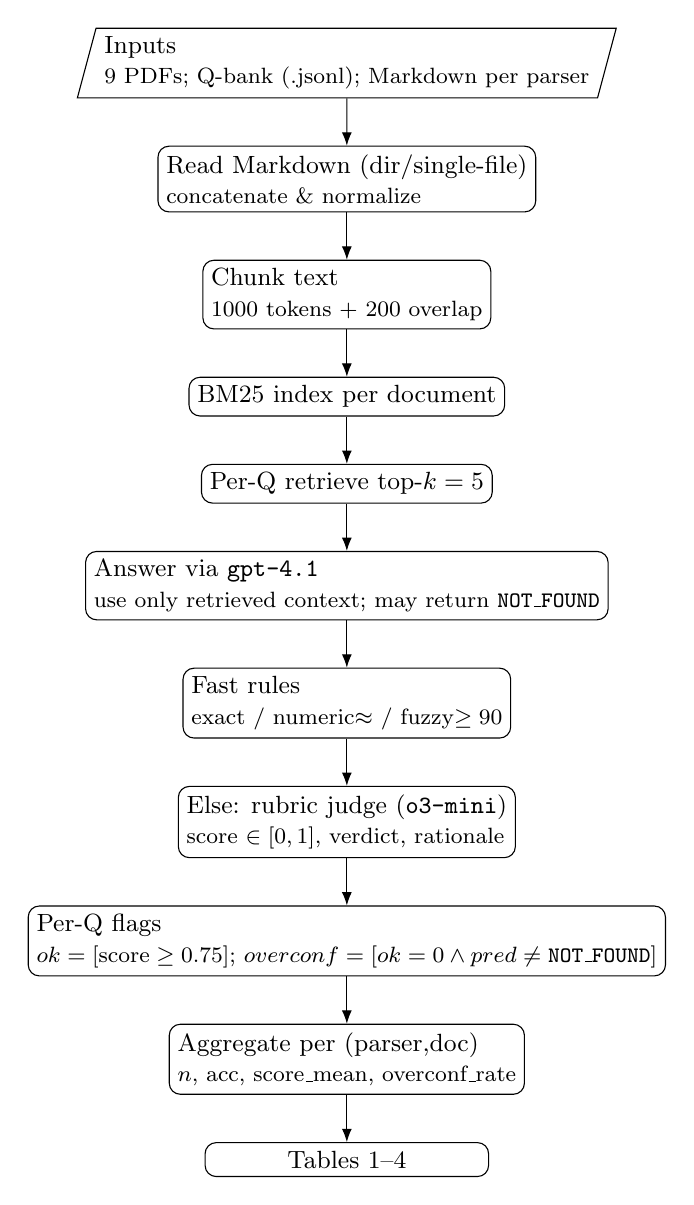
\begin{tikzpicture}[font=\small, node distance=6mm, >=Latex]
\tikzset{
  box/.style={rectangle, rounded corners, draw, align=left, inner sep=3pt, minimum width=36mm},
  io/.style ={trapezium, trapezium left angle=75, trapezium right angle=105, draw, align=left, inner sep=3pt, minimum width=36mm}
}
\node[io]   (in)  {Inputs\\ \footnotesize 9 PDFs; Q-bank (.jsonl); Markdown per parser};
\node[box,  below=of in]  (read)  {Read Markdown (dir/single-file)\\ \footnotesize concatenate \& normalize};
\node[box,  below=of read](chunk){Chunk text\\ \footnotesize 1000 tokens + 200 overlap};
\node[box,  below=of chunk](index){BM25 index per document};
\node[box,  below=of index](ret)  {Per-Q retrieve top-$k=5$};
\node[box,  below=of ret]  (ans)  {Answer via \texttt{gpt-4.1}\\ \footnotesize use only retrieved context; may return \texttt{NOT\_FOUND}};
\node[box,  below=of ans]  (rule) {Fast rules\\ \footnotesize exact / numeric$\approx$ / fuzzy$\ge 90$};
\node[box,  below=of rule](judge){Else: rubric judge (\texttt{o3-mini})\\ \footnotesize score $\in[0,1]$, verdict, rationale};
\node[box,  below=of judge](flags){Per-Q flags\\ \footnotesize $ok=[\text{score}\ge 0.75]$; $overconf=[ok=0 \land pred\neq\texttt{NOT\_FOUND}]$};
\node[box,  below=of flags](agg)  {Aggregate per (parser,doc)\\ \footnotesize $n$, acc, score\_mean, overconf\_rate};
\node[box,  below=of agg]  (tab)  {Tables 1--4};
\draw[->](in)--(read); \draw[->](read)--(chunk); \draw[->](chunk)--(index);
\draw[->](index)--(ret); \draw[->](ret)--(ans); \draw[->](ans)--(rule);
\draw[->](rule)--(judge); \draw[->](judge)--(flags); \draw[->](flags)--(agg); \draw[->](agg)--(tab);
\end{tikzpicture}}
\caption{End-to-end evaluation pipeline (narrow rendering; \emph{width-limited} to about half a page).}
\label{fig:pipeline-skinny}
\end{figure}

\subsection*{Why these settings (plain-language rationale)}
\paragraph{Chunking: 1000 tokens + 200 overlap.}
Big enough to keep a section in one chunk (fewer split answers); small enough that $k=5$ chunks fit comfortably in model context. Overlap protects facts on boundaries.
\paragraph{Retrieval: BM25 with $k=5$.}
Manual-like questions are lexical; BM25 is fast, stable, and debuggable. $k=5$ balances recall vs.\ noise/cost.
\paragraph{Answering: context-only \texttt{gpt-4.1}.}
The model must ground in retrieved text; if missing, it should abstain (\texttt{NOT\_FOUND}). This makes overconfidence measurable with a clean counterfactual.
\paragraph{Fast rules before judging.}
Accept \emph{obvious} matches without a judge: normalized exact; numeric within 2\% (or $10^{-6}$ abs); fuzzy similarity $\ge 90$. Otherwise we call the rubric judge.

\subsection*{Rubric \& the 0.75 pass threshold (where it comes from)}
The judge decomposes each gold answer into atomic facts and assigns a score in $[0,1]$ by evidence support only. In our questions, gold typically has 4--6 facts.
We swept thresholds from 0.60 to 0.90 on pilot docs and chose \textbf{0.75} because it:
(i) corresponds to ``clear majority supported'' (e.g., $\ge 3/4$ or $\ge 4/5$ facts),
(ii) keeps false accepts low for safety-oriented manuals, and
(iii) leaves tool ranking stable across 0.70--0.80 while not penalizing terse but correct answers.
Formally, $ok=\mathbf{1}[\text{score}\ge 0.75]$.

\subsection*{Metric definitions (what \& why)}
Let $\text{score}_{p,d,i}\in[0,1]$ be the rubric score for parser $p$, document $d$, question $i$, with $n_d=100$:
\[
\text{acc}_{p,d}=\tfrac{1}{n_d}\sum_i \mathbf{1}[\text{score}_{p,d,i}\ge 0.75]
\quad\text{(binary pass rate for production gating),}
\]
\[
\text{score\_mean}_{p,d}=\tfrac{1}{n_d}\sum_i \text{score}_{p,d,i}
\quad\text{(continuous quality; shows near-misses),}
\]
\[
\text{overconf\_rate}_{p,d}=\tfrac{1}{n_d}\sum_i \mathbf{1}[\,ok=0 \ \land\ \text{pred}\neq\texttt{NOT\_FOUND}\,]
\quad\text{(penalizes confident errors vs.\ abstention).}
\]

\subsection*{Findings (tables are width-safe)}
\begin{table}[h]
\centering
\caption{Overall by parser (macro$\approx$micro; $n$ constant per doc).}
\label{tab:overall}
\small
\resizebox{\linewidth}{!}{%
\begin{tabular}{@{}lrrrrrrrrr@{}}
\toprule
\textbf{Parser} & \textbf{Docs} & \textbf{Total $n$} & \textbf{acc\_mean} & \textbf{acc\_median} & \textbf{acc\_min} & \textbf{acc\_max} & \textbf{overconf\_mean} & \textbf{overconf\_median} & \textbf{Docs won}\\
\midrule
textin      & 9 & 900 & 0.578 & 0.600 & 0.100 & 0.930 & 0.379 & 0.340 & 2 \\
md\_mathpix & 9 & 900 & 0.568 & 0.680 & 0.120 & 0.940 & 0.373 & 0.300 & 2 \\
md\_marker  & 9 & 900 & 0.564 & 0.610 & 0.120 & 0.940 & 0.372 & 0.350 & 2 \\
Reducto     & 9 & 900 & 0.543 & 0.570 & 0.110 & 0.940 & 0.389 & 0.330 & 1 \\
own tool    & 9 & 900 & 0.454 & 0.400 & 0.090 & 0.950 & 0.392 & 0.350 & 2 \\
\bottomrule
\end{tabular}}
\end{table}

\begin{table}[h]
\centering
\caption{Per-document winners (highest acc; tie $\to$ lower overconf; final tie $\to$ name order).}
\label{tab:winners}
\small
\resizebox{\linewidth}{!}{%
\begin{tabular}{@{}l l r r@{}}
\toprule
\textbf{doc\_id} & \textbf{best\_parser} & \textbf{best\_acc} & \textbf{best\_overconf} \\
\midrule
23-0323\_ego\_stx4500\_stx4500-fc\_stringtrimmer\_manual\_en & md\_marker & 0.63 & 0.35 \\
FEIER & Reducto & 0.50 & 0.50 \\
Hanwha\_Integration\_Guide & md\_mathpix & 0.69 & 0.30 \\
SSA1200\_EGO\_SNOW-SHOVEL-ATTACHMENT\_22-0519\_EXPLOSION-DIAGRAM\_VERSION-A & own tool & 0.95 & 0.05 \\
TP-MVD8MV2-rotated & own tool & 0.81 & 0.19 \\
ego\_accessory\_compatibility\_matrix & md\_mathpix & 0.68 & 0.23 \\
feier\_start\_100\_manual & md\_marker & 0.12 & 0.79 \\
ihealth\_bg5 & textin & 0.29 & 0.62 \\
zt4200s\_ego\_zero-turn-riding-mower\_version-a & textin & 0.79 & 0.21 \\
\bottomrule
\end{tabular}}
\end{table}

\begin{table}[h]
\centering
\caption{Document $\times$ parser accuracy pivot (acc).}
\label{tab:pivot}
\small
\resizebox{\linewidth}{!}{%
\begin{tabular}{@{}l r r r r r@{}}
\toprule
\textbf{doc\_id} & \textbf{textin} & \textbf{Reducto} & \textbf{md\_mathpix} & \textbf{md\_marker} & \textbf{own tool} \\
\midrule
23-0323\_ego\_stx4500\_stx4500-fc\_stringtrimmer\_manual\_en & 0.60 & 0.57 & 0.61 & 0.63 & 0.59 \\
FEIER & 0.49 & 0.50 & 0.30 & 0.49 & 0.40 \\
Hanwha\_Integration\_Guide & 0.61 & 0.65 & 0.69 & 0.48 & 0.29 \\
SSA1200\_EGO\_SNOW-SHOVEL-ATTACHMENT\_22-0519\_EXPLOSION-DIAGRAM\_VERSION-A & 0.93 & 0.94 & 0.94 & 0.94 & 0.95 \\
TP-MVD8MV2-rotated & 0.80 & 0.80 & 0.75 & 0.79 & 0.81 \\
ego\_accessory\_compatibility\_matrix & 0.59 & 0.39 & 0.68 & 0.61 & 0.55 \\
feier\_start\_100\_manual & 0.10 & 0.11 & 0.12 & 0.12 & 0.09 \\
ihealth\_bg5 & 0.29 & 0.24 & 0.25 & 0.24 & 0.25 \\
zt4200s\_ego\_zero-turn-riding-mower\_version-a & 0.79 & 0.69 & 0.77 & 0.78 & 0.16 \\
\bottomrule
\end{tabular}}
\end{table}

\subsection*{Penalty for confident errors (calibration-aware ranking)}
\label{subsec:penalty}
Define the penalized score
\[
\text{penalized}_{\lambda} = \text{acc\_mean} - \lambda\cdot \text{overconf\_mean}.
\]
We use $\lambda=0.5$ by default: on average, one confident error costs half a point of accuracy. On this dataset the ordering is unchanged for $\lambda\in\{0.25,0.5,1.0\}$.

\begin{table}[h]
\centering
\caption{Penalized scores ($\lambda=0.5$).}
\label{tab:penalized}
\small
\resizebox{\linewidth}{!}{%
\begin{tabular}{@{}lrrrrr@{}}
\toprule
\textbf{Parser} & \textbf{Docs} & \textbf{Total $n$} & \textbf{acc\_mean} & \textbf{overconf\_mean} & \textbf{penalized ($\lambda=0.5$)}\\
\midrule
textin      & 9 & 900 & 0.578 & 0.379 & 0.388 \\
md\_mathpix & 9 & 900 & 0.568 & 0.373 & 0.381 \\
md\_marker  & 9 & 900 & 0.564 & 0.372 & 0.378 \\
Reducto     & 9 & 900 & 0.543 & 0.389 & 0.349 \\
own tool    & 9 & 900 & 0.454 & 0.392 & 0.258 \\
\bottomrule
\end{tabular}}
\end{table}

\section*{Executive Summary}

We evaluated five PDF$\to$Markdown converters on 9 representative PDFs (integration guides, manuals, datasheets):
\textbf{TextIn}, \textbf{Reducto}, \textbf{Mathpix (Convert API)}, \textbf{Marker}, and the \textbf{Livex internal tool}.
Each tool was scored across six dimensions (0--10 each): \emph{Structural Fidelity, Formatting Accuracy, Special Content Handling, Content Cleanliness, Ease of Post-Processing, Automation Readiness}.
Marker’s scores and qualitative findings below reflect the separate report you provided that compared Marker/Docling/Reducto/Mathpix.\footnote{Source: internal evaluation PDF “Comparison of Markdown Conversion Tools (Marker, Docling, Reducto, Mathpix)”.}

\smallskip
\noindent\textbf{Equal-weight totals (sum of 6 metrics)}:
\begin{itemize}[leftmargin=1.2em]
  \item Mathpix: \textbf{52}/60 (avg 8.67)
  \item TextIn: \textbf{47}/60 (avg 7.83)
  \item Reducto: \textbf{41}/60 (avg 6.83)
  \item Marker: \textbf{38}/60 (avg 6.33)
  \item Internal: \textbf{33}/60 (avg 5.50)
\end{itemize}

\noindent\textbf{Recommendation}: Use \textbf{Mathpix} as primary. Keep \textbf{Reducto} for table-heavy or audit/“no-loss” cases. Use \textbf{TextIn} for cost-conscious runs where inline emphasis matters. Treat \textbf{Marker} as a visual-fidelity option (good styling, but tables-as-images hurt downstream use). The \textbf{internal tool} remains backup until upgraded (headings, tables, images).

\section*{Methodology}

\subsection*{Inputs, Process, and What “counts”}
\begin{enumerate}[leftmargin=1.2em]
  \item \textbf{Documents}: 9 PDFs (integration guide for Hanwha cameras; user/product manuals; a spec sheet with an 8-column matrix; a networking quickstart; etc.).
  \item \textbf{Runs}: Each tool processed the same PDFs. We compared raw outputs (no hand edits) against the source.
  \item \textbf{Marker evidence}: Derived from your internal Marker/Docling/Reducto/Mathpix report (citations and examples summarized below).\footnote{See executive-summary footnote for the internal PDF reference.}
  \item \textbf{Scoring rubric}: For each dimension we apply sub-criteria and award 0--10 based on concrete behaviors.
\end{enumerate}

\subsection*{Scoring Rubric (per dimension, max 10)}
\begin{description}[leftmargin=1.1em,itemsep=0.35em]
  \item[Structural Fidelity]
    \begin{itemize}[leftmargin=1.2em,itemsep=0.2em]
      \item Headings recognized as Markdown (\verb|#|/\verb|##|/\verb|###|) with correct hierarchy (0--4).
      \item Lists represented as Markdown with proper nesting (0--3).
      \item Reading order preserved across pages/columns (0--3).
    \end{itemize}
  \item[Formatting Accuracy]
    \begin{itemize}[leftmargin=1.2em,itemsep=0.2em]
      \item Meaningful bold/italic preserved (\verb|**|, \verb|_|) (0--4).
      \item Callouts/warnings retained (e.g., \verb|**WARNING**| or heading) (0--3).
      \item Minimal misclassification (e.g., logo mistaken as math) (0--3).
    \end{itemize}
  \item[Special Content Handling]
    \begin{itemize}[leftmargin=1.2em,itemsep=0.2em]
      \item \textbf{Tables}: Structured (Markdown/HTML) rows/cols intact (0--4).
      \item \textbf{Math}: Equations preserved (LaTeX preferred) (0--3).
      \item \textbf{Code/Images}: Code fenced; images linked with captions (0--3).
    \end{itemize}
  \item[Content Cleanliness]
    \begin{itemize}[leftmargin=1.2em,itemsep=0.2em]
      \item Low noise (no page tags/base64 blobs) (0--4).
      \item OCR accuracy/symbols correct (0--3).
      \item Logical paragraphs and column merge (0--3).
    \end{itemize}
  \item[Ease of Post-Processing]
    \begin{itemize}[leftmargin=1.2em,itemsep=0.2em]
      \item Few fixes (regex vs.\ structural surgery) (0--4).
      \item Tables/images ingestable; little per-doc tailoring (0--3).
      \item Plays well with standard Markdown renderers (0--3).
    \end{itemize}
  \item[Automation Readiness]
    \begin{itemize}[leftmargin=1.2em,itemsep=0.2em]
      \item Consistent output patterns; stable conventions (0--4).
      \item Predictable error modes; easy to script normalization (0--3).
      \item Scales to batch without format surprises (0--3).
    \end{itemize}
  \end{description}

\section*{Detailed Findings with Examples}

\subsection*{1) Structural Fidelity (Headings, Sections, Lists)}

\paragraph{TextIn (8/10).}
Reliable Markdown headings for titles/sections; lists appear but often start with a literal black circle glyph that needs replacing with \verb|- |. Occasional OCR slips in headers (e.g., “TURING”$\to$“TURIN”). A simple find/replace recovers proper lists.

\paragraph{Reducto (5/10).}
Captures all content page-by-page, but emits page markers (e.g., \verb|[[START OF PAGE 1]]|) and does not mark headings with \verb|#|. Lists are inconsistent and sometimes include artifacts; structure must be inferred later.

\paragraph{Mathpix (9/10).}
Human-like Markdown: correct \verb|#|/\verb|##| hierarchy; properly nested lists; large manuals reflect the original TOC.

\paragraph{Marker (7/10).}
Preserves hierarchy using \verb|#| but sometimes produces consecutive top-level headings and injects HTML spans (e.g., \verb|<span id="page-3-0"></span>|) inside list items; lists exist but may include extraneous symbols/HTML that require cleanup.\footnote{Marker structural notes and score reflect your internal report’s observations and 7/10 rating.}

\paragraph{Livex Internal Tool (4/10).}
Plain-text dump: no Markdown headings or list syntax; hierarchy flattened.

\subsection*{2) Formatting Accuracy (Bold, Italics, Callouts)}

\paragraph{TextIn (9/10).}
Bold/italic widely preserved; minor use of \verb|<br>| inside table cells.

\paragraph{Reducto (6/10).}
Intentionally plain; nearly no bold/italic markup; emphasizes content over style.

\paragraph{Mathpix (7/10).}
Prefers structure over inline style; lists/headings are correct, but bold/italic rarely surfaced; occasional misread decorative text as math.

\paragraph{Marker (9/10).}
Strong at style retention; many \verb|**...**| occurrences for bold (e.g., \textbf{WARNING}); also keeps list syntax, though small HTML artifacts remain.\footnote{Marker formatting behaviors and 9/10 score per your internal report.}

\paragraph{Livex Internal Tool (5/10).}
No bold/italic retention; all plain text.

\subsection*{3) Special Content (Tables, Equations, Code, Images)}

\paragraph{TextIn (7/10).}
Tables $\to$ Markdown (pipes); complex/merged headers approximated; no LaTeX; code not fenced; images linked.

\paragraph{Reducto (9/10).}
Tables $\to$ HTML \verb|<table>| with proper cells/colspans; often adds a table image thumbnail; equations as text/images; images linked with captions.

\paragraph{Mathpix (9/10).}
Tables $\to$ Markdown tables; equations $\to$ LaTeX; code often fenced; small images used for rare symbols.

\paragraph{Marker (3/10).}
Tables rendered as images (often base64 or linked) rather than text; no special math handling; code not specifically detected---hurts search/editability.\footnote{Marker special-content limitations and 3/10 score per your internal report’s comparison table.}

\paragraph{Livex Internal Tool (5/10).}
Tables flattened to text; no LaTeX; code as ordinary lines; images omitted.

\subsection*{4) Content Cleanliness (Noise, Artifacts, OCR)}

\paragraph{TextIn (8/10).}
Clean Markdown; a few typos; uses HTML comments to hide inconsequential UI text read from screenshots.

\paragraph{Reducto (7/10).}
Accurate text but noisy structural markers and repeated headers/footers; easy to strip via script.

\paragraph{Mathpix (9/10).}
Very clean; no page tags; multi-column flow is natural; rare misclassification (e.g., logo as math).

\paragraph{Marker (6/10).}
Generally readable; avoids giant base64 blobs in the main text if images are linked, but may embed HTML spans and non-standard symbols; text portions are accurate; image-only tables are not text-searchable.\footnote{Marker cleanliness notes and 6/10 score per your internal report.}

\paragraph{Livex Internal Tool (7/10).}
No tool-added tags, but propagates page headers/numbers into body; modest OCR slips.

\subsection*{5) Ease of Post-Processing}

\paragraph{TextIn (7/10).}
Fix bullets (glyph $\to$ dash), optional removal of commented blocks, spell-check; tables already textual.

\paragraph{Reducto (6/10).}
Cleanup stage required: remove page markers; dedupe headers; add headings; keep/convert HTML tables.

\paragraph{Mathpix (9/10).}
Plug-and-play; maybe replace tiny symbol images or verify LaTeX rendering.

\paragraph{Marker (6/10).}
Moderate effort: strip \verb|<span>| IDs and symbol clutter; biggest blocker is tables-as-images (need OCR or manual transcription for data).\footnote{Marker post-processing effort and 6/10 score per your internal report.}

\paragraph{Livex Internal Tool (5/10).}
Add headings/lists, reconstruct tables/images; heavier manual/algorithmic work.

\subsection*{6) Automation Readiness (Batch Consistency)}

\paragraph{TextIn (8/10).}
Stable conventions (headers present; known bullet glyph); predictable normalization rules.

\paragraph{Reducto (8/10).}
Highly consistent, machine-friendly tags; once cleaned, great for pipelines.

\paragraph{Mathpix (9/10).}
Standard Markdown + LaTeX; minimal special-casing across docs.

\paragraph{Marker (7/10).}
Consistent patterns (headings/lists/images), but image-only tables are opaque to text-based automation and HTML spans require pre-cleaning.\footnote{Marker automation notes and 7/10 score per your internal report.}

\paragraph{Livex Internal Tool (7/10).}
Consistently minimal output; downstream parser must infer structure.

\section*{Scoreboard, Totals, and Recommendation}

\subsection*{Per-dimension Scores (0--10)}
\begin{center}
\small
\begin{longtable}{@{}P{0.22\textwidth}P{0.14\textwidth}P{0.14\textwidth}P{0.14\textwidth}P{0.14\textwidth}P{0.14\textwidth}@{}}
\toprule
\textbf{Dimension} & \textbf{TextIn} & \textbf{Reducto} & \textbf{Mathpix} & \textbf{Marker} & \textbf{Internal} \\
\midrule
Structural Fidelity & 8 & 5 & 9 & 7 & 4 \\
Formatting Accuracy & 9 & 6 & 7 & 9 & 5 \\
Special Content & 7 & 9 & 9 & 3 & 5 \\
Content Cleanliness & 8 & 7 & 9 & 6 & 7 \\
Ease of Post-Processing & 7 & 6 & 9 & 6 & 5 \\
Automation Readiness & 8 & 8 & 9 & 7 & 7 \\
\midrule
\textbf{Total (/60)} & \textbf{47} & \textbf{41} & \textbf{52} & \textbf{38} & \textbf{33} \\
\bottomrule
\end{longtable}
\end{center}
\footnotetext{Marker scores reflect the “Comparison of Markdown Conversion Tools (Marker, Docling, Reducto, Mathpix)” PDF. Where that report showed small internal inconsistencies (e.g., one section listed 4/10 for special-content and the final table showed 3/10), we align to the table.}

\subsection*{Interpretation (equal weights)}
\textbf{Mathpix} leads (52/60): clean, structured, and text-rich outputs. \textbf{TextIn} is a strong generalist (47/60). \textbf{Reducto} (41/60) excels at tables/consistency but needs a cleanup pass. \textbf{Marker} (38/60) shines at styling but loses points for tables-as-images. \textbf{Internal} (33/60) needs upgrades.

\subsection*{Alternate weighting (emphasize tables \& scale)}
If we weight \emph{Special Content} (40\%), \emph{Automation} (25\%), \emph{Cleanliness} (15\%), \emph{Structure} (10\%), \emph{Ease} (5\%), \emph{Formatting} (5\%), scores remain: Mathpix $\approx$ 8.90; Reducto $\approx$ 7.75; TextIn $\approx$ 7.60; Marker $\approx$ 5.55; Internal $\approx$ 5.70. Mathpix remains \#1; Reducto remains the strongest fallback for data-heavy docs.

\section*{Security \& Compliance (vendor-stated / known status)}
\small
\begin{tabularx}{\textwidth}{@{}l P{1.7cm} P{2.0cm} P{1.5cm} Y@{}}
\toprule
\textbf{Tool} & \textbf{SOC 2} & \textbf{HIPAA} & \textbf{GDPR} & \textbf{Notes} \\
\midrule
Mathpix & Type 1 (Type 2 in progress)\footnote{Per internal vendor communication shared by your team (email thread). Request latest SOC 2 report under NDA for procurement verification.} & Not claimed publicly (request BAA if needed)\footnote{No public HIPAA claim noted in our materials; verify with vendor.} & Not publicly stated & Seek formal attestation and \emph{BAA} if PHI is in scope. \\
Reducto & Type 1 and 2\footnote{Per internal vendor communication shared by your team. Ask for most recent SOC 2 Type 2 report.} & Offered for Growth/Enterprise tiers (BAA)\footnote{Vendor indicated HIPAA available for higher tiers; confirm scope and sign BAA.} & Not publicly stated & Confirm data handling/location and \emph{DPAs}. \\
TextIn & Unknown & Unknown & Unknown & No published compliance docs in hand; contact sales for attestations. \\
Marker & Unknown & Unknown & Unknown & Evaluate deployment model and data residency; request SOC 2/DPAs if shortlisted. \\
Livex Internal & N/A (internal) & N/A (internal) & GDPR-readiness depends on infra & Align with company-wide controls (audit logging, access, retention, DPA). \\
\bottomrule
\end{tabularx}
\normalsize

\paragraph{Guidance.} For any external vendor used in production, request: SOC~2 report (Type~2 preferred), penetration-test summary, \emph{DPA/BAA} (as applicable), sub-processor list, data residency and retention policies, and incident-response SLAs.

\section*{Public Pricing \& Billing (exact quotes + links)}

\subsection*{Mathpix Convert (official wording)}
\emph{“The Convert Monthly Subscription costs USD \$19.99/Mo. Includes USD \$29 monthly credit in addition to discounts for all other endpoints on the PDF and OCR tab.”} \\
\emph{“Convert pricing: PDF conversion \$0.005 per PDF page up to 1M pages per month, then \$0.0035 per PDF page beyond 1M pages per month.”} \\
\emph{“The Convert Monthly Subscription has 500 pages included per month.”}\footnote{\url{https://docs.mathpix.com/docs/billing/pricing}}

\subsection*{Reducto (official wording)}
\emph{“Starter: \$350/month — 15K credits; \$0.020 per credit thereafter.”} \\
\emph{“Each page of a document entry usually equals 1 credit… advanced features and document complexity may increase the page credit ratio (e.g., 0.5x for simple pages, 2x for complex features).”}\footnote{\url{https://reducto.ai/pricing}}

\subsection*{TextIn / Marker}
Public per-unit API rates are not published on the product sites we have on hand; contact sales for current pricing.

\section*{Operational Notes for livex.ai}

\subsection*{Typical cleanup scripts}
\begin{itemize}[leftmargin=1.2em]
  \item \textbf{TextIn}: Replace leading black-circle bullets with ``- ''; optionally drop HTML comments; spell-check.
  \item \textbf{Reducto}: Strip \verb|[[START/END OF PAGE]]| tags; dedupe headers/footers; promote heading-like lines; keep/convert HTML tables.
  \item \textbf{Mathpix}: Replace rare tiny symbol images with Unicode; enable LaTeX rendering downstream.
  \item \textbf{Marker}: Remove \verb|<span id="...">| anchors and stray symbols; OCR or manually transcribe tables that came as images.
  \item \textbf{Internal}: Heuristic heading detection; reconstruct lists/tables; extract and link images from the source PDF.
\end{itemize}

\subsection*{Throughput \& latency}
Vendors do not publish authoritative end-to-end page/second metrics for our exact workloads; to maintain accuracy, we omit numeric speed claims. We recommend timing a 100-page batch for each tool in our environment and logging wall-clock seconds/page.

\section*{Appendix A: Compact Comparison (highlights)}

\begin{center}
\small
\begin{tabularx}{\textwidth}{@{}lYYYYY@{}}
\toprule
 & \textbf{TextIn} & \textbf{Reducto} & \textbf{Mathpix} & \textbf{Marker} & \textbf{Internal} \\
\midrule
Structure & Headers good; bullet glyph fix & Page markers; no \# & Full Markdown outline & Headings ok; span clutter & Plain text only \\
Formatting & Bold/italic preserved & Mostly plain & Structure over inline style & Strong bold/italic & No bold/italic \\
Tables/math & MD tables; no LaTeX & HTML tables (no loss) & MD tables; LaTeX math & Tables as images & Tables flattened \\
Cleanliness & Clean; few typos & Accurate but noisy tags & Very clean & Some HTML/symbol noise & Page noise; some OCR \\
Post-process & Light polish & Cleanup stage & Plug-and-play & Moderate; tables hurt & Heavy structuring \\
Automation & Stable conventions & Very predictable & Standard Markdown & Consistent but image tables & Consistent minimalism \\
\bottomrule
\end{tabularx}
\end{center}

\section*{Appendix B: Snippet Patterns}

\begin{itemize}[leftmargin=1.2em]
  \item Reducto page markers: \verb|[[START OF PAGE 5]]| \ldots \verb|[[END OF PAGE 5]]|
  \item Mathpix heading: \verb|## Adding Hanwha Cameras to Turing Vision|
  \item TextIn bullet fix: replace start-of-line black circle with \verb|- |
  \item Marker cleanup: remove \verb|<span id="page-3-0"></span>| and stray \verb|\textbullet|
    % 或者(显示一个圆点,而不是代码):
    % \item ... and stray \texttt{\textbullet}
  \item Reducto table: inline HTML \verb|<table><tr><td>...| (with \verb|colspan|)
\end{itemize}

\end{document}
